% !TeX spellcheck = <none>
\chapter{Voorstelling van het stagebedrijf}
\vspace{-3cm}
\section{Ontstaan en geschiedenis}
Engagor werd opgericht in 2011 door Folke Lemaitre (ex-werknemer van Netlog) met de bedoeling interactie met klanten, via sociale media, te vereenvoudigen. Sinds 2015 maakt Engagor deel uit van Clarabridge. Dit Amerikaanse bedrijf ontwikkelt software om automatisch online data te verzamelen, te categoriseren en te rapporteren. Gebruikelijk is dit data verkregen van sociale media zoals Facebook en Twitter. Maar andere platformen zoals YouTube, Instagram, Vimeo en Tumbler kunnen ook beheerd worden. Kort samengevat zijn ze dus gespecialiseerd in software voor Customer Experience Management (CEM). Het gaat hier dus vooral om feedback over interacties die plaatsvinden tussen de klanten en het bedrijf. Zo kunnen bedrijven hun strategie aanpassen om hun klanten zo goed mogelijk van dienst te zijn \cite{bp1}. Tegenwoordig is sociale media niet meer weg te denken uit het dagelijkse leven, noch bij particulieren noch bij bedrijven. Dit resulteert in een zeer groot klantenbestand met grote klanten zoals Telenet, NMBS, AirBnb, Ikea en Turkish Airlines.

Na de overname werd Engagor onderdeel van CX Social (CX staat hier voor Consumer Experience), een van de vier producten van Clarabridge. De andere drie zijn CX Survey, CX Studio en CX Designer. Met CX Survey kunnen surveys aangemaakt en verwerkt worden. De verwerking van surveys gebeurt onder andere met behulp van tekst en sentiment analyse. CX Studio is een \textit{dashboarding tool} waarmee gebruikers hun CEM proces kunnen stroomlijnen. Als laatste is er ook nog CX Designer dat voor data modellering gebruikt wordt \cite{Clarabridge.com}. 

Clarabridge heeft momenteel ongeveer 250 werknemers, verspreid over de hele wereld. Het hoofdkantoor bevindt zich in Reston, Virginia, Amerika. Maar er zijn kantoren in Gent, Larkspur (California), Londen, Barcelona en Singapore \cite{ClarabridgeOffices}. Op elk van deze locaties en in India zijn \textit{support teams} aanwezig. Zo kunnen ze 24/5 en in sommige gevallen zelfs 24/7, hun klanten bijstaan.

Voor mijn stage werk ik aan CX Social. Dit is dus de \textit{customer care tool} voor sociale media. Gebruikers kunnen via de webapplicatie snel en gemakkelijk antwoorden op vragen en/of klachten op hun sociale profielen zoals Facebook, Twitter en Instagram. Dit is voor grote bedrijven natuurlijk zeer handig aangezien zij dagelijks gigantisch veel berichten (zowel priv\'{e}berichten als \textit{posts}) op hun profielen moeten verwerken. E\'{e}n gemeenschappelijke plaats waaruit alle profielen kunnen onderhouden worden, is dus onontbeerlijk. 

\begin{figure}[H]
	\centering
	
\includegraphics[width=0.6\textwidth]{Figuren/CXSocialLogo.png}
	\caption{CX Social Logo \cite{CXSOcialLogo}} 
	\label{fig:CXSocialLogo}
\end{figure} 

Het CXSocial team bestaat uit ongeveer 35 werknemers. Zij werken constant aan het verbeteren en onderhouden van deze \textit{tool}.  Binnen het team werken de meesten als \textit{Full stack software engineer}. Zij werken dus zowel aan de backend van de webapplicatie als aan de API en frontend. Het team wordt vervolledigd door mensen die zich bezighouden met \textit{data science} en design. \textit{Data scientists} werken onder andere met \textit{machine learning} en statistieken. Het belang hiervan valt in een sociale media \textit{monitoring tool} niet te onderschatten. Ook het design is zeer belangrijk tijdens het ontwikkelen van een webapplicatie. Telkens een nieuw \textit{feature} toegevoegd wordt, wordt hiervan een ontwerp gemaakt om dit nieuwe stukje zo goed mogelijk in het geheel te implementeren. De designers moeten er natuurlijk ook voor zorgen dat hun ontwerpen overeenkomen met alle producten die Clarabridge aanbiedt. Ook moet alles wat ze ontwerpen zo gebruiksvriendelijk mogelijk gemaakt worden \cite{EngagorTeam}. 

Wanneer nieuwe \textit{features} ge\"{i}mplementeerd moeten worden, wordt dit ofwel door \'{e}\'{e}n iemand uitgewerkt of door enkele personen uit het team. Tijdens het ontwikkelen kan feedback en hulp van collega`s ingeroepen worden waardoor iedereen altijd betrokken is bij verschillende projecten. Dit zorgt er voor dat niet enkel degene die het project toegewezen krijgt, weet hoe alles in elkaar zit. Zo is iedereen op elk moment op de hoogte van veranderingen aan de \textit{code base}. 

Op Figuur~\ref{fig:Organigram} is de organisatie binnen het CX Social team te zien. Dit organigram is niet volledig accuraat want de positie van Solutions Engineer moet hier nog aan toegevoegd worden maar het schept een zeer goed beeld van de verschillende functies binnen CX Social. 

\begin{figure}[H]
	\centering
	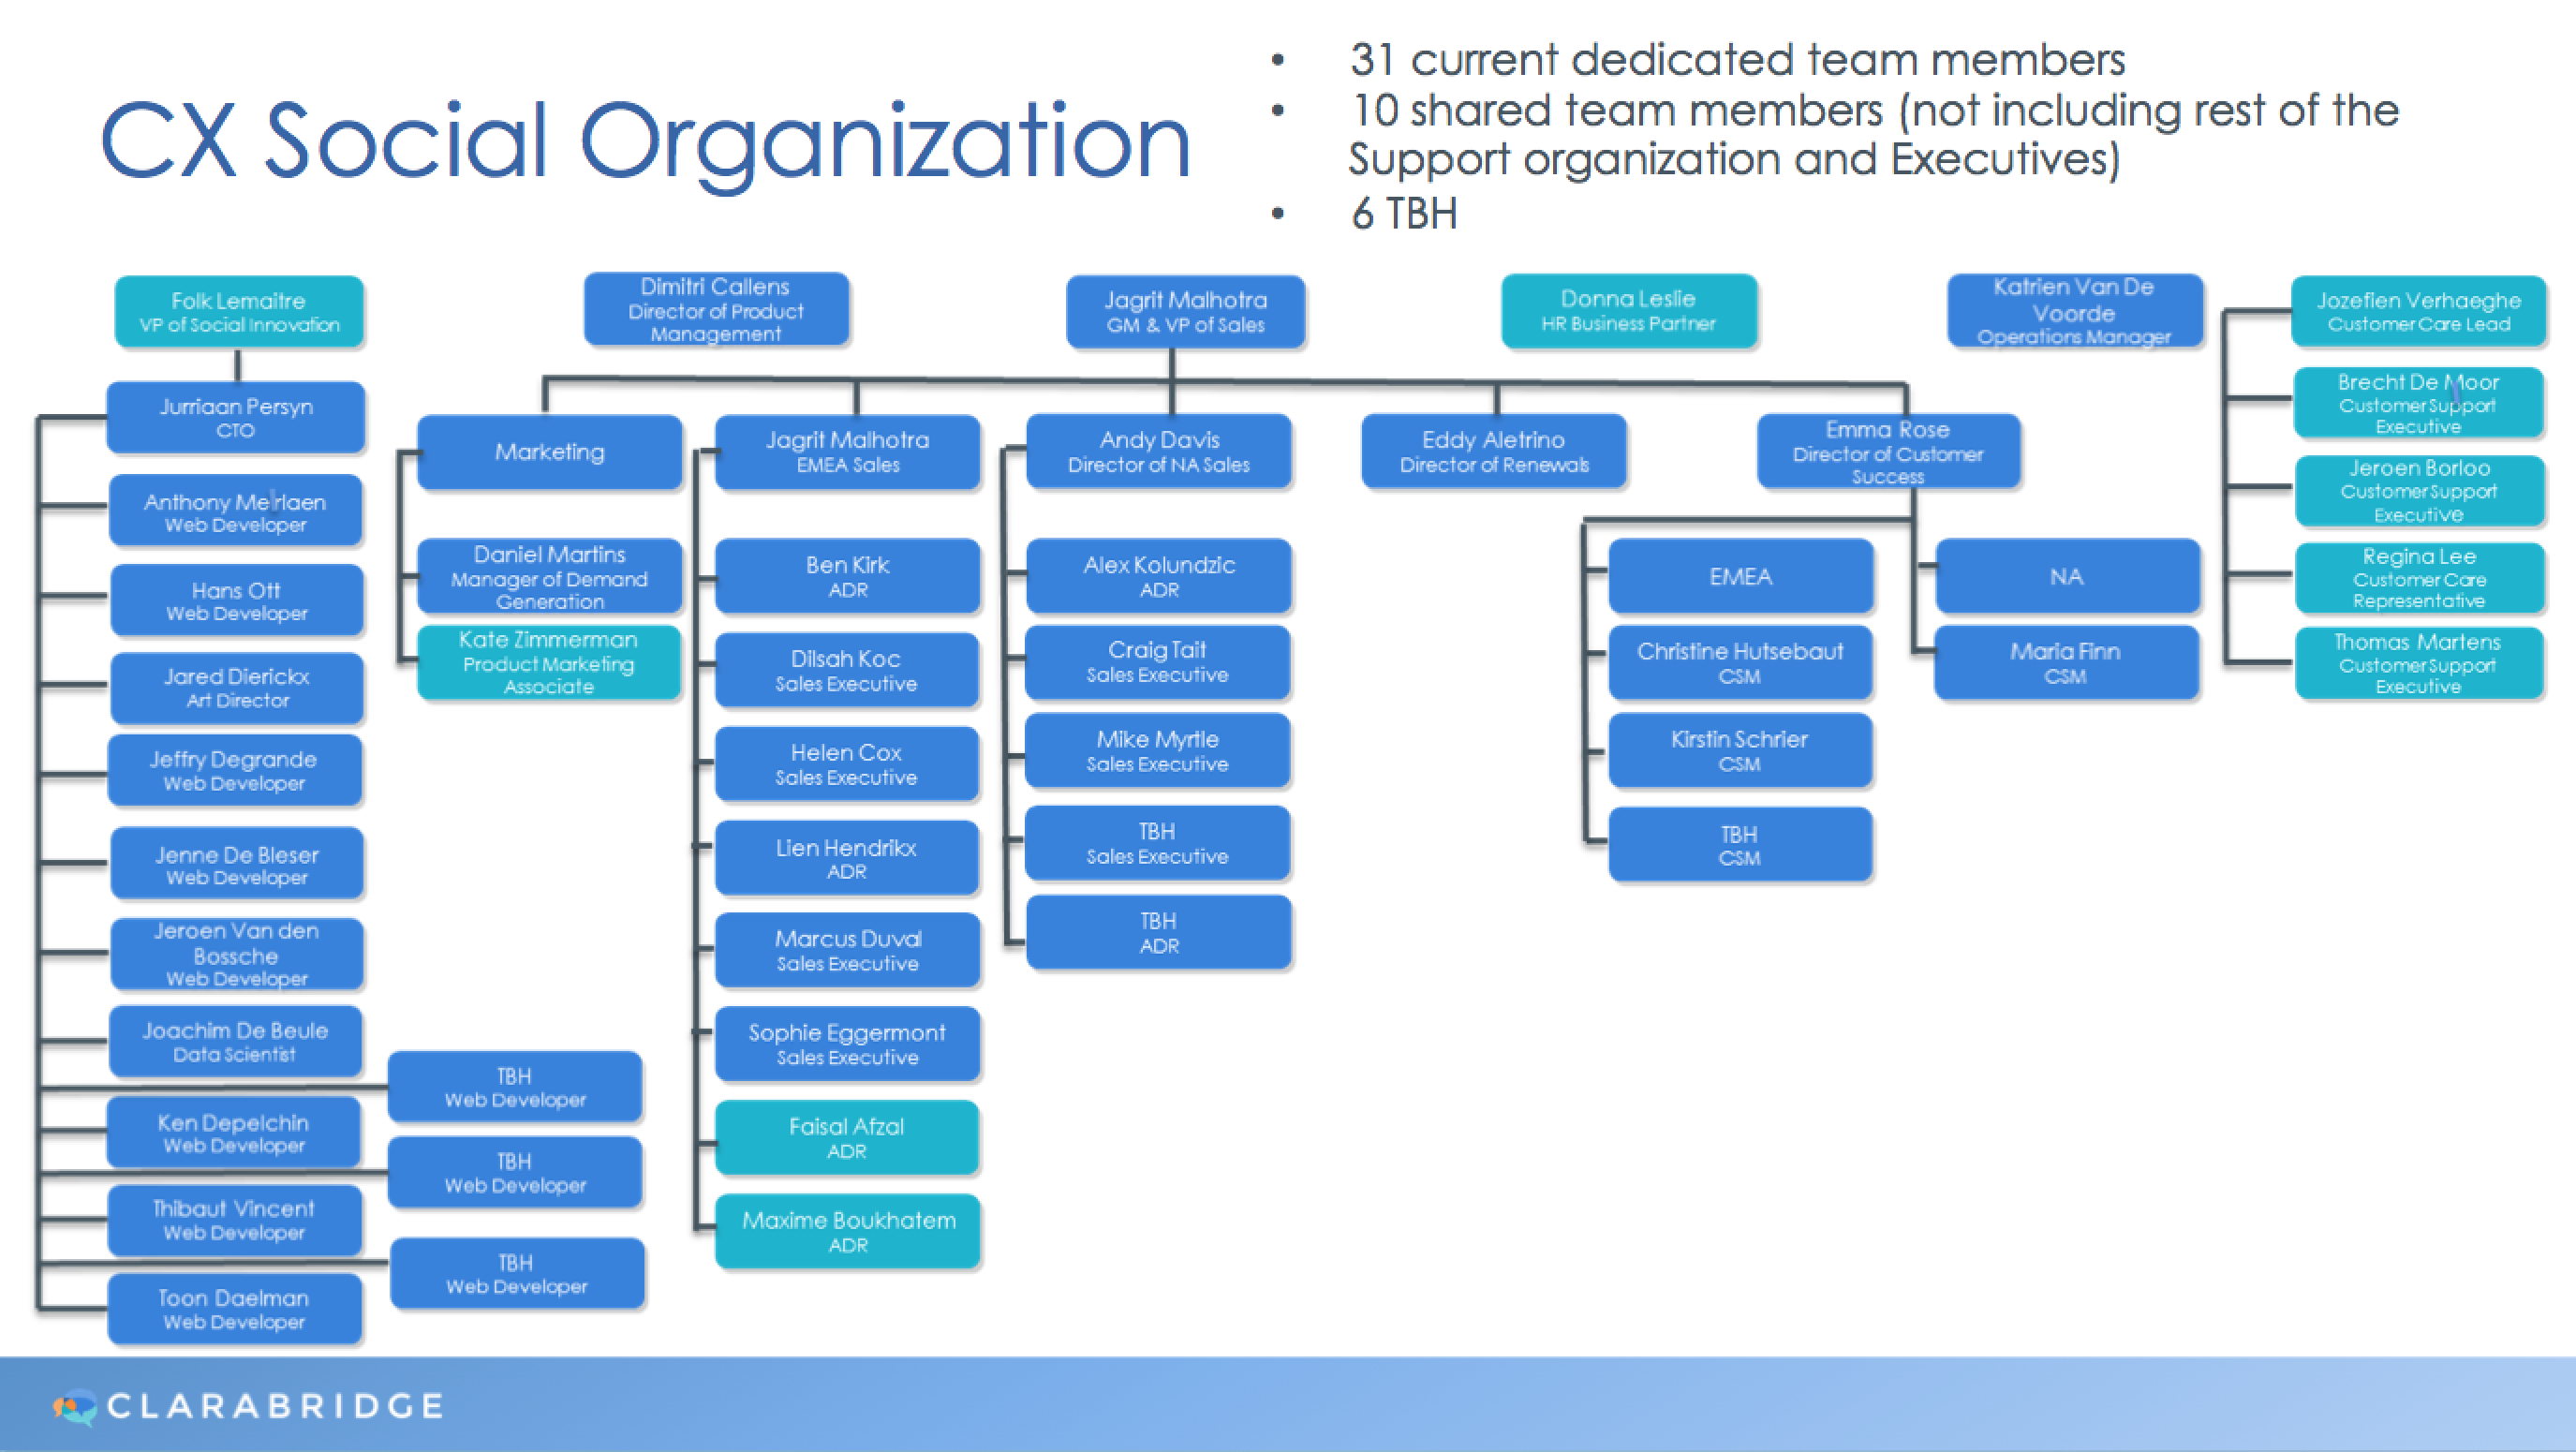
\includegraphics[width=1\textwidth]{Figuren/Organigram.png}
	\caption{Organigram CX Social \cite{Jagrit}} 
	\label{fig:Organigram}
\end{figure} 

\section{CX Social} \label{CXSocial}
Elk product, aangeboden door Clarabridge, is toegespitst op de analyse van customer feedback. CX Social is de sociale media \textit{monitoring}, management en analyse tool die gebruikt wordt door verschillende grote bedrijven om hun klanten beter te ondersteunen. Het principe van de \textit{tool} is dat op \'{e}\'{e}n gemeenschappelijke plaats verschillende profielen beheerd kunnen worden. Zo kunnen onder meer berichten van klanten beantwoord worden, statistieken bekeken worden of kan de inhoud van de profielen aangepast worden. 

Engagor maakt in hun webapplicatie gebruik van PHP, JavaScript, HTML en CSS. Het grootste deel is geschreven in PHP met het DooPHP \textit{framework}. Dit \textit{framework} is momenteel niet meer in ontwikkeling maar werd aangepast voor gebruik binnen de Engagor webapplicatie waardoor verdere ontwikkeling van DooPHP door de ontwikkelaars niet onmiddellijk nodig is \cite{DooPHP}. %Naast PHP en JavaScript frameworks wordt ook gebruik gemaakt van MySQL, Redis, memcached, ElasticSearch en RabbitMQ. 

In de frontend wordt vooral gebruik gemaakt van React (ook gekend als React.js/ReactJS). Dit is een open-source JavaScript bibliotheek, ontwikkeld door Facebook, waarmee zeer gemakkelijk interfaces aangemaakt kunnen worden. Met React kunnen componenten gecre\"{e}erd worden, waarin wordt vastgelegd wat gerenderd moet worden voor de gebruiker. React zal ervoor zorgen dat de componenten effici\"{e}nt en correct ge\"{u}pdatet worden wanneer data verandert. Aan deze componenten kunnen ook parameters meegegeven worden en op basis hiervan kunnen views aan de gebruiker getoond worden \cite{React}. 

CX Social is dus, zoals eerder vermeld, een sociale media \textit{monitoring}, management en analyse tool. Zo kunnen klanten op de webapplicatie een centrale inbox raadplegen (zie Bijlage, Figuur~\ref{fig:Inbox}). Hier worden berichten per profiel verzameld en kunnen medewerkers reageren op de vragen/opmerkingen van klanten.
 
\iffalse
\begin{figure}[H]
	\centering
	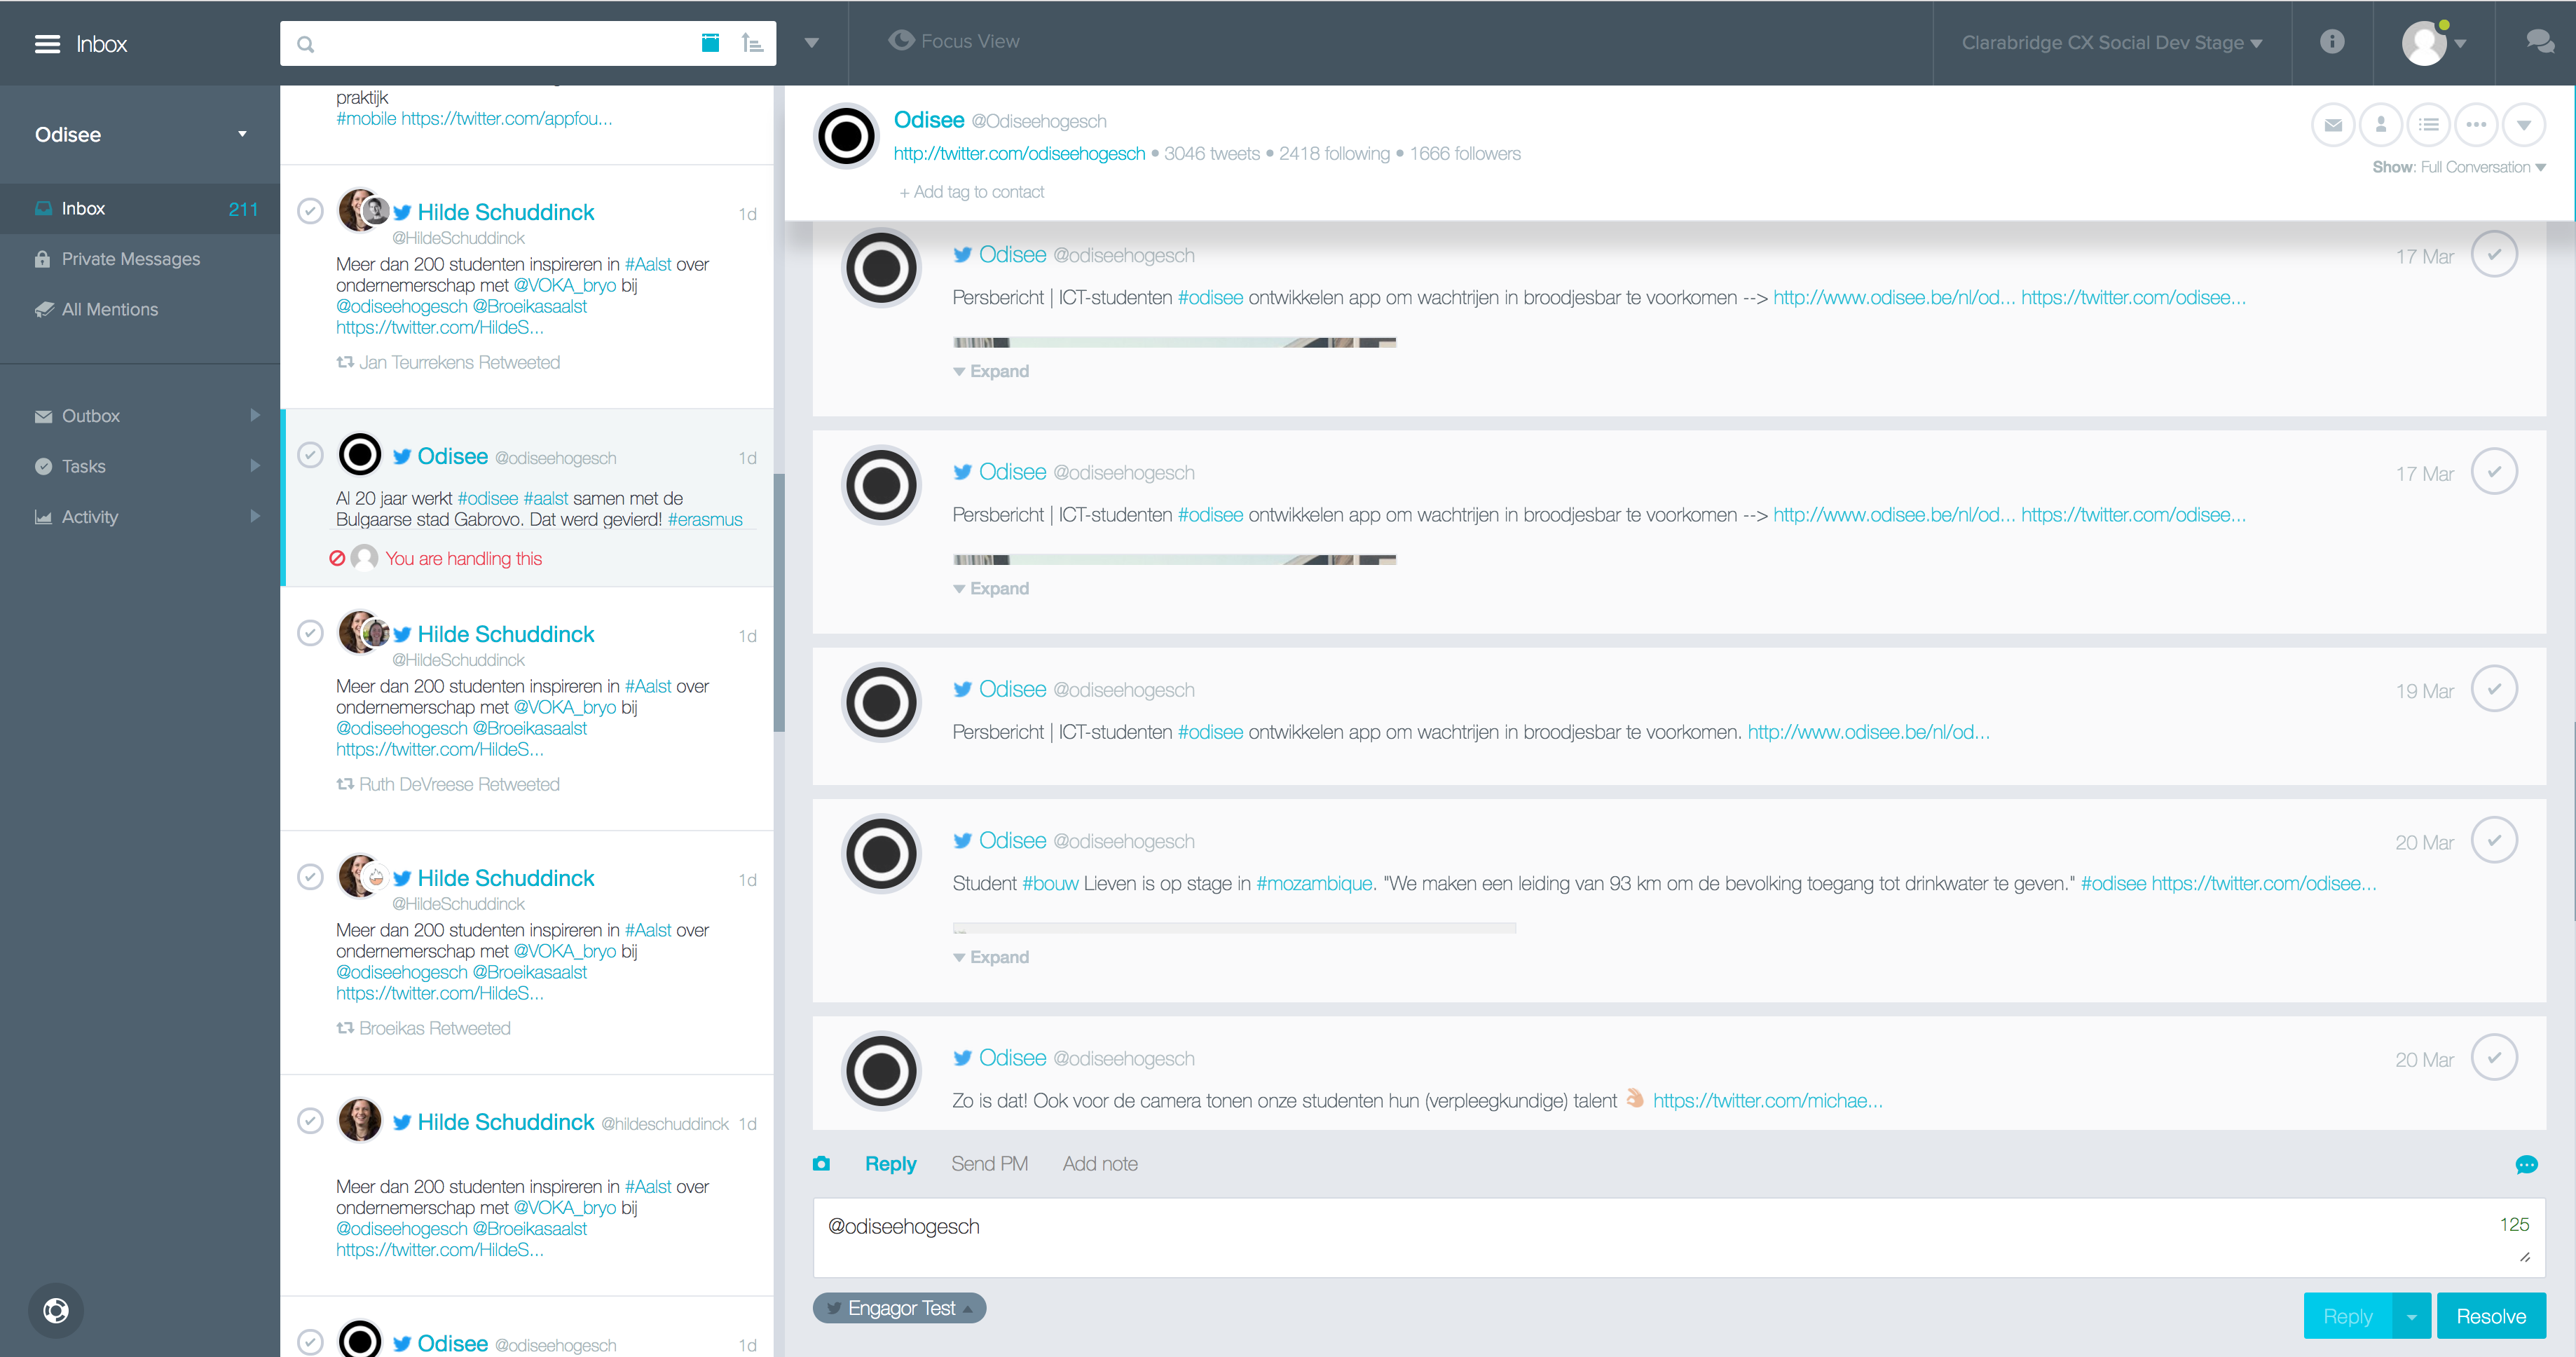
\includegraphics[width=1\textwidth]{Figuren/Inbox.png}
	\caption{Inbox CX Social \cite{EngagorScreenshots}} %\cite{Pouladzadeh}
	\label{fig:Inbox}
\end{figure} 
\fi

Via de `Performance' pagina kunnen bedrijven de statistieken van hun pagina's bijhouden. Hier is bijvoorbeeld te zien hoe lang het duurde voor actie werd ondernomen, hoeveel unieke gebruikers geholpen werden of hoeveel antwoorden gemiddeld gegeven werden op een \textit{mention} (zie Bijlage, Figuur~\ref{fig:Performance}).

Meer statistieken zijn terug te vinden op de `Insights' pagina. Zo zijn de totale mentions van een \textit{topic} te zien alsook de \textit{mentions} per pagina. Dit alles wordt zeer intu\"{i}tief  weergegeven in de vorm van cirkeldiagrammen en tijdlijnen. Hier wordt ook het sentiment berekend. Dit geeft een aanduiding van het percentage van de mentions die een positieve, negatieve of neutrale connotatie hebben. Ook trends (veelgebruikte woorden, hashtags  etc.) en foto's die binnen een topic voorkomen zijn hier te vinden (zie Bijlage, Figuur~\ref{fig:Insights}).  



\iffalse
Via de `Insights' kunnen bedrijven ook de statistieken van hun pagina's bijhouden. Zo zijn de totale mentions van een \textit{topic} te zien alsook de \textit{mentions} per pagina. Dit alles wordt zeer intu\"{i}tief  weergegeven in de vorm van cirkeldiagrammen en tijdlijnen. Hier wordt ook het sentiment berekend. Dit geeft een aanduiding van het percentage van de mentions die een positieve, negatieve of neutrale connotatie hebben. Ook trends (veelgebruikte woorden, hashtags  etc.) en foto's die binnen een topic voorkomen zijn hier te vinden (zie Bijlage, Figuur~\ref{fig:Insights}).  


\begin{figure}[H]
	\centering
	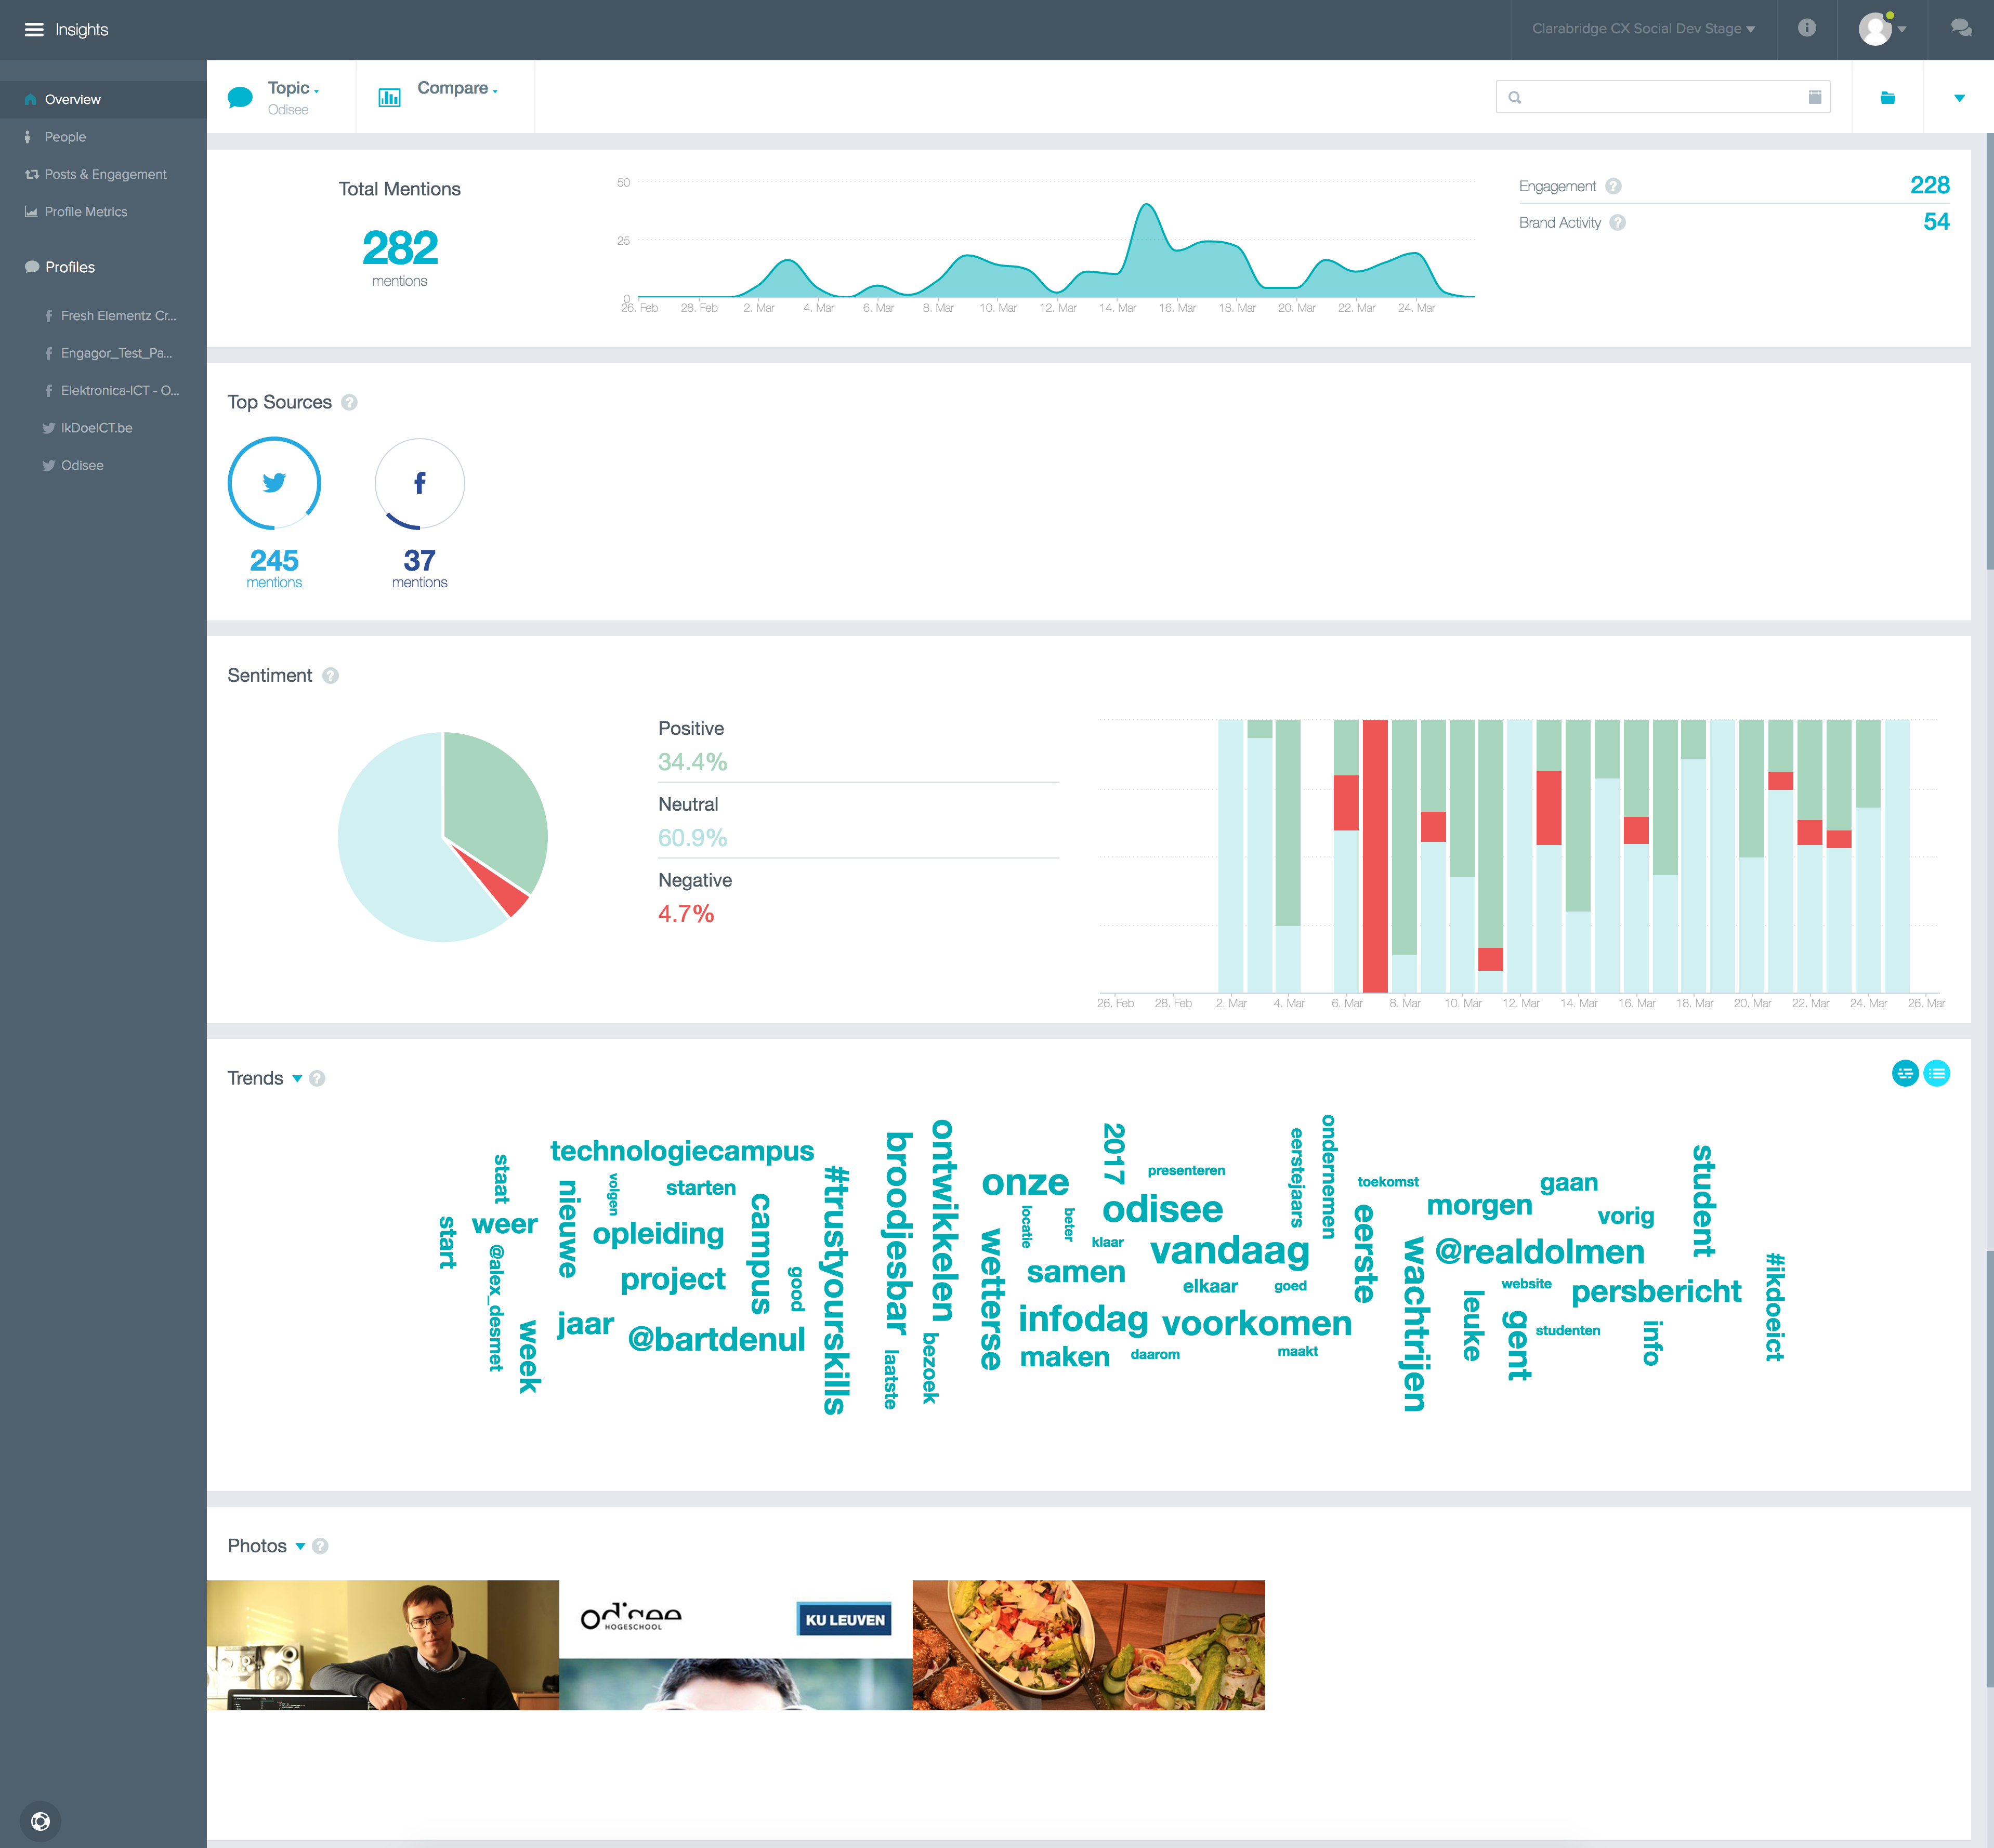
\includegraphics[width=1\textwidth]{Figuren/Insights.png}
	\caption{Insights CX Social \cite{EngagorScreenshots}} %\cite{Pouladzadeh}
	\label{fig:Insights}
\end{figure} 
\fi

\iffalse
Nog meer statistieken zijn terug te vinden op de `Performance' pagina. Hier is bijvoorbeeld te zien hoe lang het duurde voor actie werd ondernomen, hoeveel unieke gebruikers geholpen werden of hoeveel antwoorden gemiddeld gegeven werden op een mention (zie Bijlage, Figuur~\ref{fig:Performance}).

\begin{figure}[H]
	\centering
	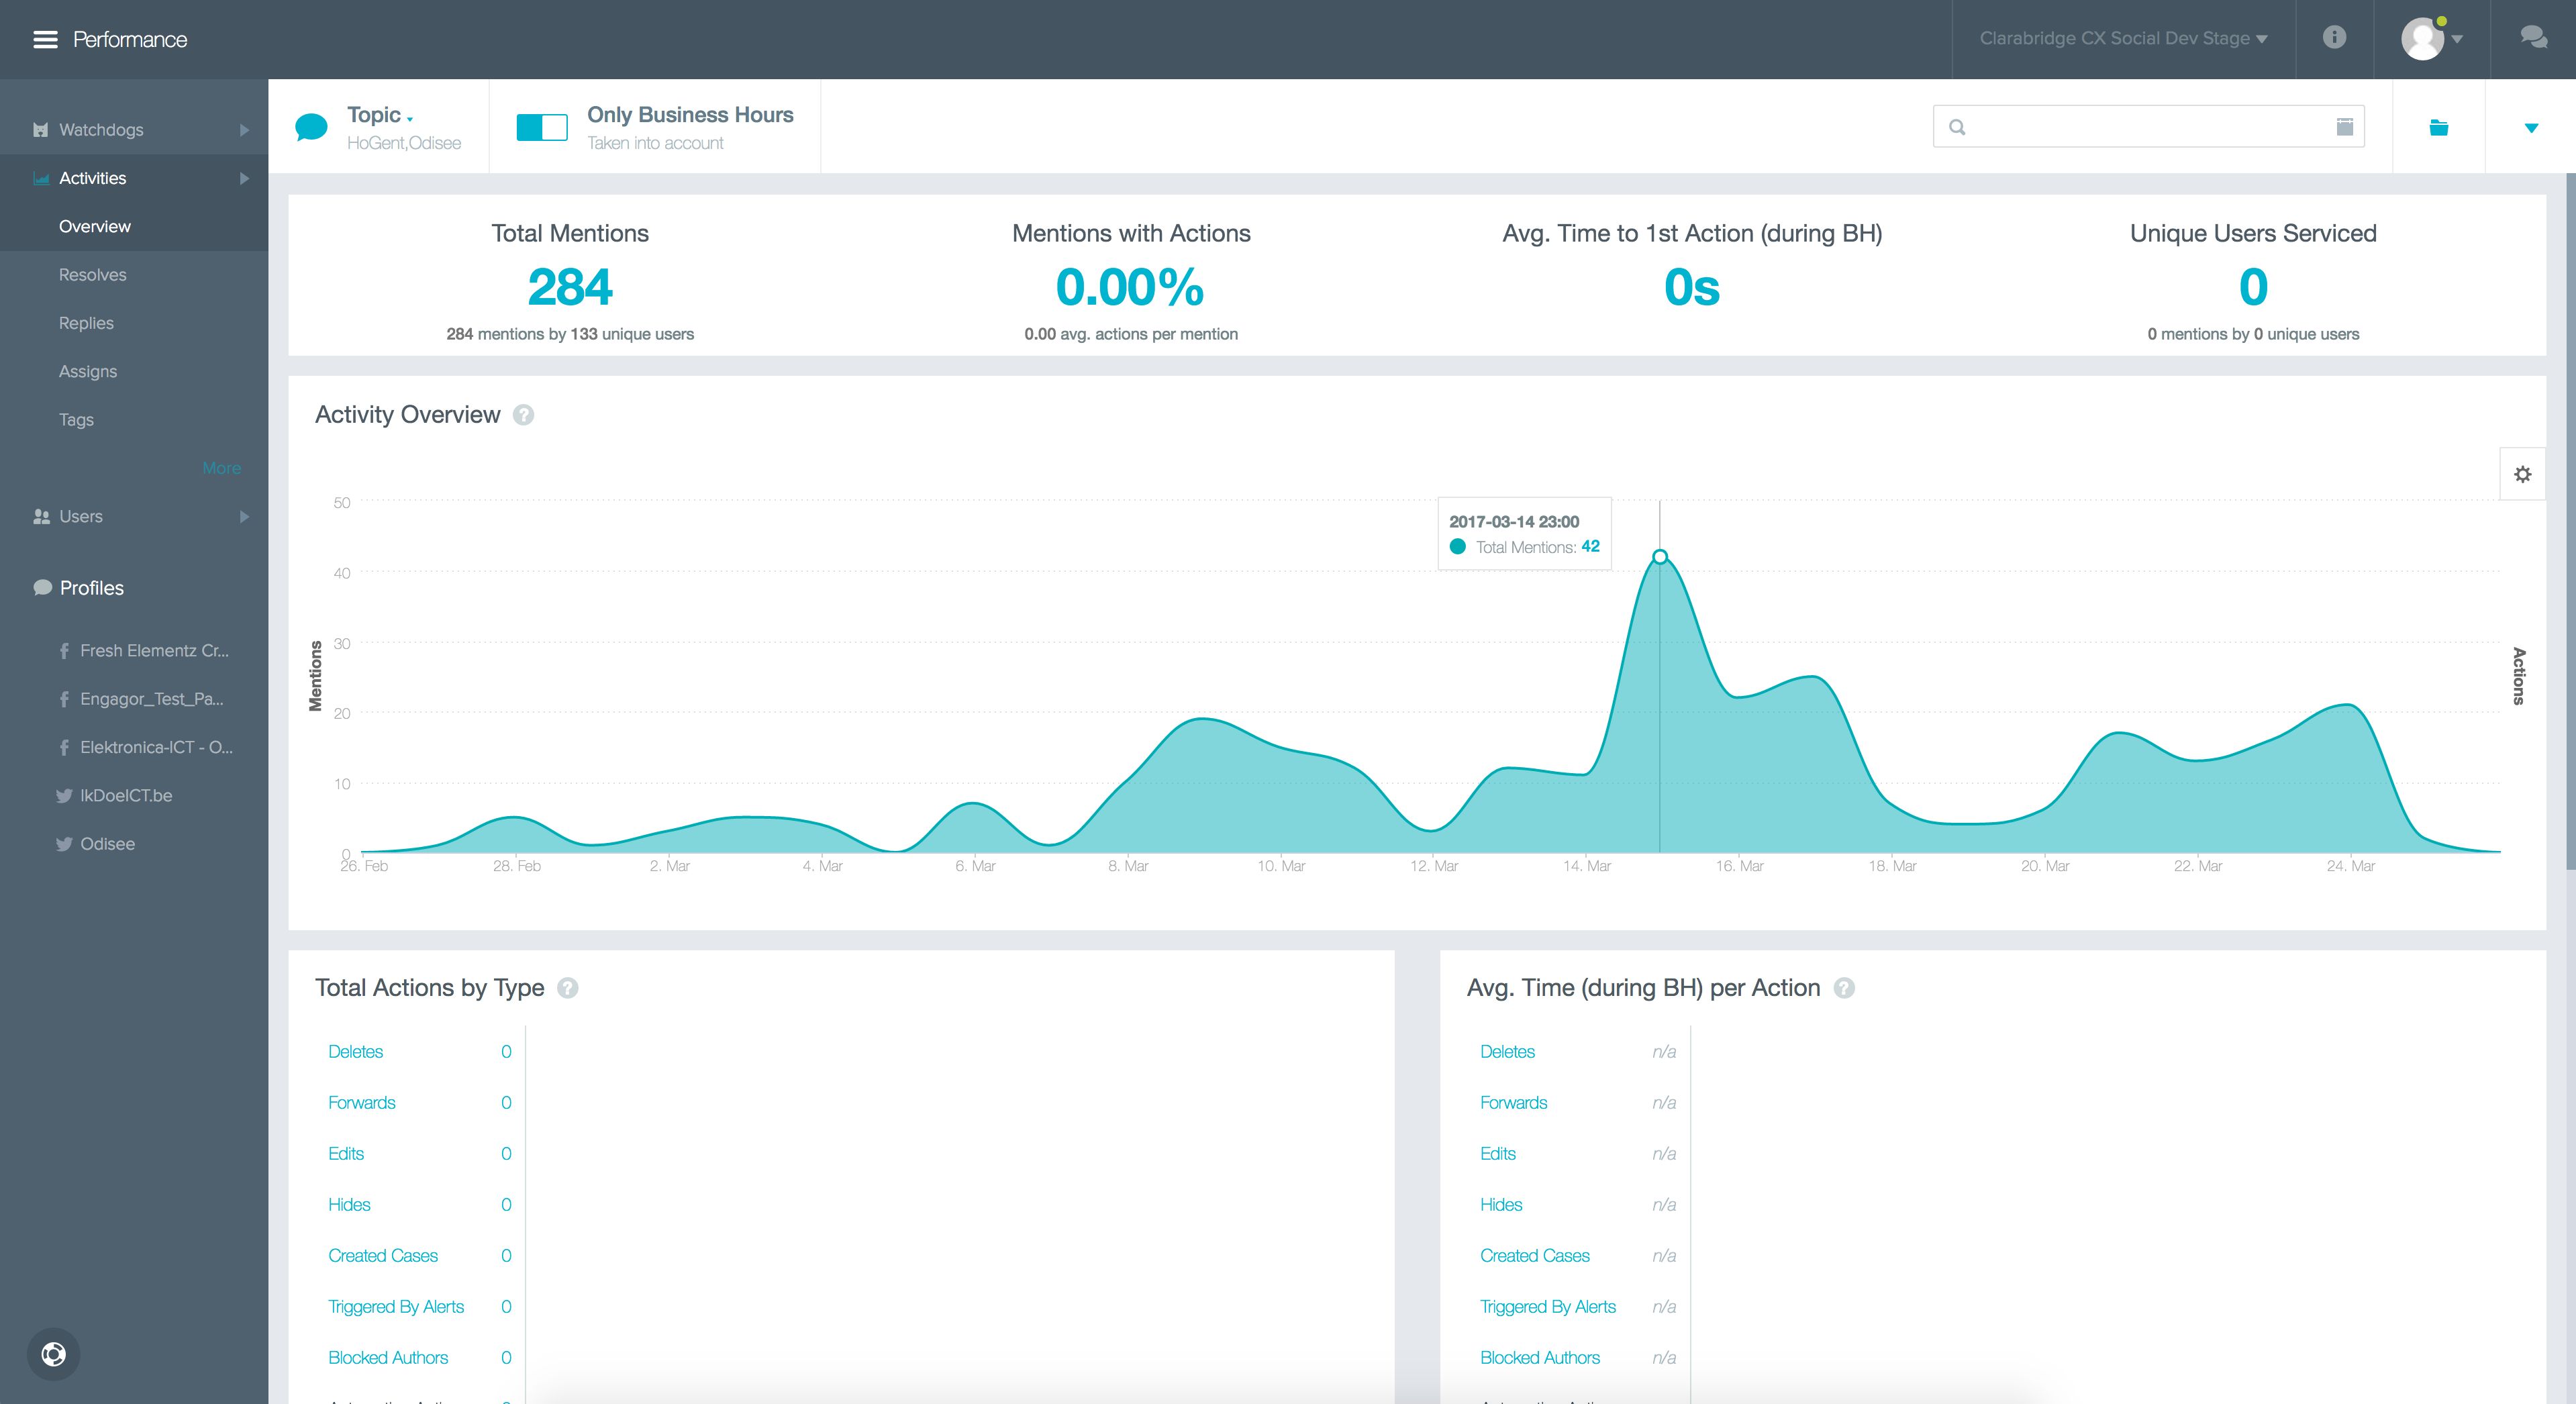
\includegraphics[width=1\textwidth]{Figuren/Performance.png}
	\caption{Performance CX Social \cite{EngagorScreenshots}} %\cite{Pouladzadeh}
	\label{fig:Performance}
\end{figure} 
\fi


Niet enkel berichten kunnen beheerd worden via de webapplicatie maar er kan ook gepost worden op profielen zelf. Dit kan per topic en per profiel gebeuren. Posts kunnen ook gepland worden om ze op een later tijdstip op het profiel weer te geven  of opgeslagen worden als \textit{canned response}. Dit zijn standaard antwoorden die gebruikt kunnen worden tijdens het communiceren met klanten \cite{EngagorApp}. Zo kunnen klanten sneller geholpen worden met hun problemen.
 
\chapter{Probleemstelling}
\vspace{-3cm}
\section{Probleemstelling vanuit de stage} \label{BeschrijvingStageOpdracht}

Als stageopdracht dient een nieuwe feature toegevoegd te worden aan de CX Social webapplicatie: een \textit{profile manager}. Deze \textit{profile manager} moet gebruikers in staat stellen de profielfoto en/of omslagfoto van een profiel in te stellen. Dit gebeurt aan de hand van thema's. Een thema kan aangemaakt worden voor een specifieke service, bijvoorbeeld Facebook of Twitter. Voor Facebook kan een thema een omslagfoto en een profielfoto bevatten terwijl een thema voor Twitter naast de foto's ook de link kleur kan bevatten (zie Figuur~\ref{fig:EditTheme}). Het moet ook mogelijk zijn voor de klanten om deze afbeeldingen aan te passen. Zo kunnen ze tekst toevoegen aan de afbeelding of hun eigen \textit{Key Performance Indicator} (KPI)\footnote{Een \textit{Key Performance Indicator} is een meetbare waarde waarmee de prestaties van bedrijven of ondernemingen uitgedrukt worden. Binnen CX Social zijn dit bijvoorbeeld de geholpen klanten per dag of hoe lang het gemiddeld duurt voor klanten geholpen worden} er op plaatsen. Aangezien de omslagfoto's van Facebook en Twitter niet dezelfde dimensies bezitten en de foto ook niet op volledige grootte aan de gebruikers kan getoond worden, zullen de afbeeldingen ook herschaald moeten worden naar de correcte dimensies.

\begin{figure}[H]
	\centering
	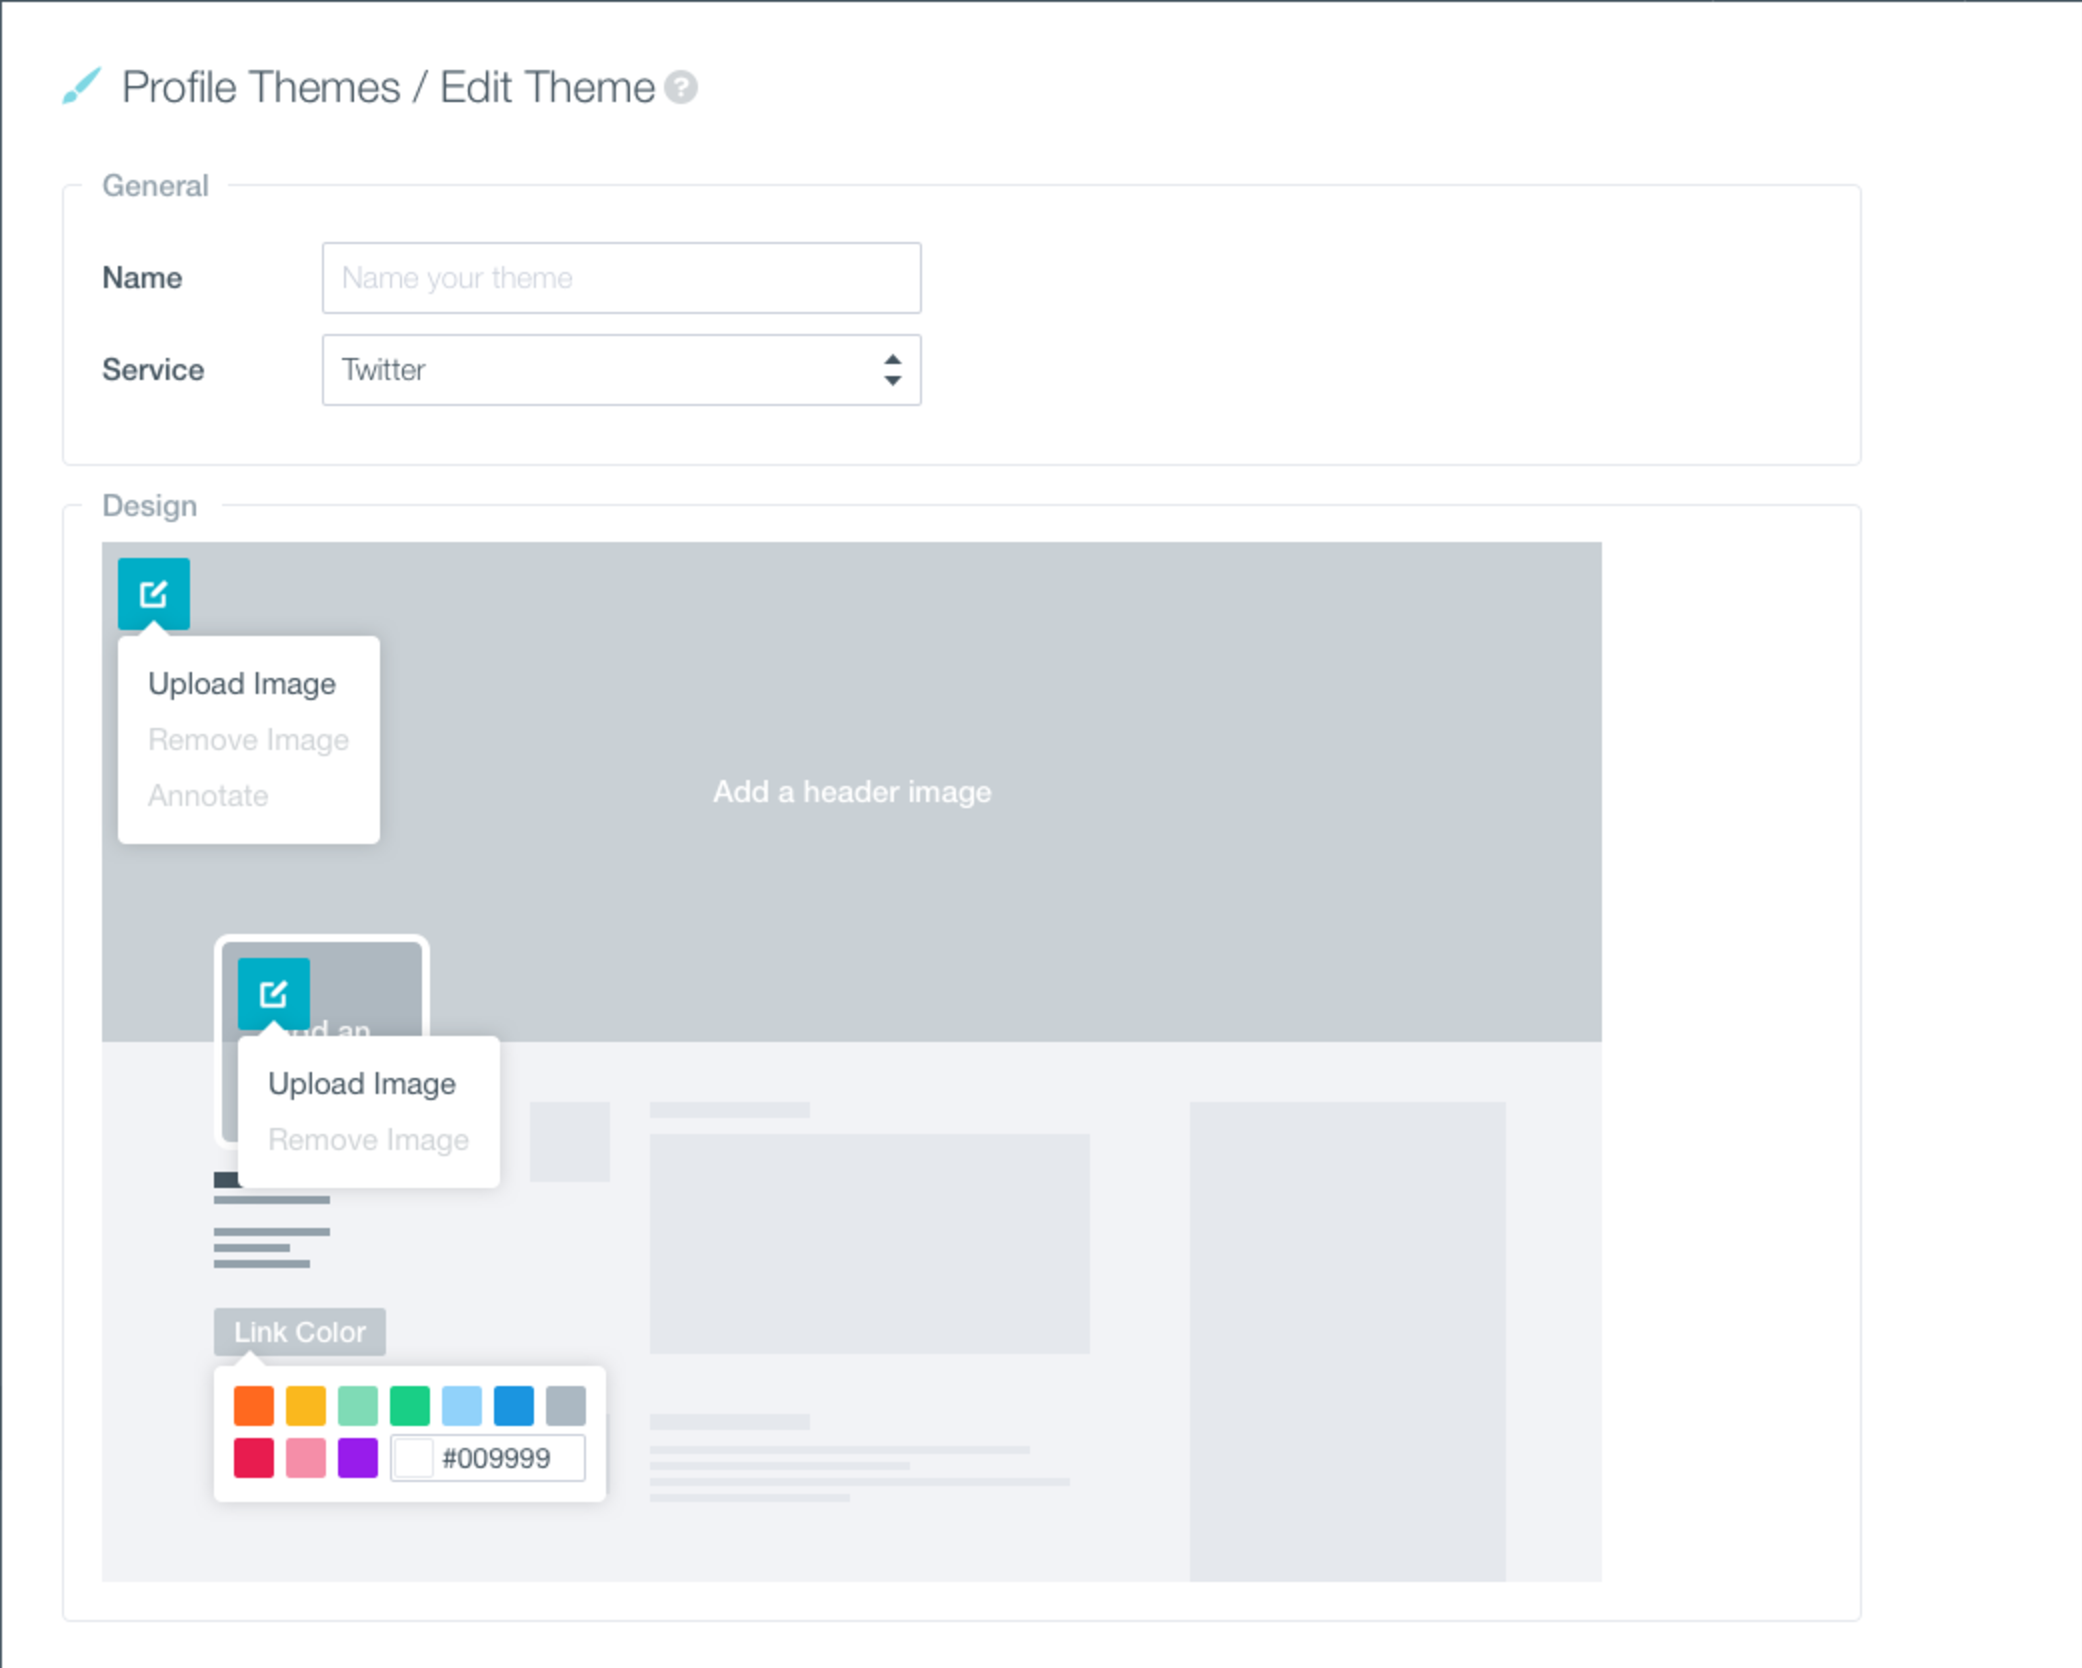
\includegraphics[width=0.7\textwidth]{Figuren/EditThemeMockup.png}
	\caption{Mockup van de editeerpagina \cite{EditThemeMockup}} %\cite{Pouladzadeh}
	\label{fig:EditTheme}
\end{figure} 

Verschillende thema's moeten aan een planning toegevoegd kunnen worden. Een klant kan dan instellen dat een bepaald thema ofwel binnen de \textit{business hours} gebruikt wordt ofwel tijdens een bepaalde periode ofwel tijdens beide. Een speciaal thema voor bijvoorbeeld Kerstmis kan dan ingesteld worden om tijdens de kerstperiode zichtbaar te zijn op het profiel. Wanneer meerdere thema's op een profiel zijn ingesteld, moet dus berekend worden welk van deze thema's op een gegeven moment toegepast moet worden. 

\newpage
De webapplicatie bezit ook \textit{Crisis Plans}. Dit zijn instellingen die bij een probleem binnen het bedrijf actief gesteld kunnen worden. Eens actief wordt een waarschuwing getoond, rechten van gebruikers veranderd of een to-do lijstje opgesteld met stappen die ondernomen moeten worden om het probleem op te lossen. Via een \textit{Crisis Plan} moet ook een thema ingesteld kunnen worden. Een gebruiksscenario hiervoor zou bijvoorbeeld kunnen zijn: het instellen van een specifieke omslagfoto en avatar wanneer een bedrijf kampt met een technische storing. 

\section{Probleemstelling bachelorproef}

Deel van de stageopdracht is het verwerken van afbeeldingen om als omslagfoto of avatar te gebruiken. Hierbij is het de bedoeling dat klanten afbeeldingen kunnen uploaden die dan als omslagfoto en/of avatar zullen dienen. Een thema, bestaande uit deze afbeeldingen en in sommige gevallen nog enkele andere variabelen zoals link kleur voor een Twitter profiel, kunnen ingesteld worden om op bepaalde tijdstippen actief te zijn. Klanten moeten in staat zijn tekst en KPI's op deze afbeeldingen te plaatsen vanuit de webapplicatie. De afbeeldingen moeten dus samengesteld kunnen worden door de gebruiker maar moeten nadien ook opnieuw gegenereerd kunnen worden op de server met aangepaste KPI's. 

Om afbeeldingen te annoteren is redelijk wat functionaliteit vereist. Ingegeven tekst moet eender waar op een afbeelding geplaatst kunnen worden maar moet ook gestyled kunnen worden. Lettertype, kleur, lettergrootte, gewicht en uitlijning moeten allemaal ingesteld kunnen worden door gebruikers. Dit alles moet zowel clientside als serverside mogelijk zijn aangezien de KPI's telkens zullen veranderen waardoor nieuwe afbeeldingen gegeneerd moeten worden. 

Naast het genereren van de afbeeldingen moeten deze ook ge\"{u}pload worden naar Facebook of Twitter op de ingestelde tijdstippen. Er moet dus geregeld berekend worden welke afbeelding met welke KPI's op een bepaald tijdstip ingesteld moet worden als omslagfoto. De gebruiker verwacht natuurlijk dat telkens de correcte foto, inclusief up-to-date KPI's, op het profiel ingesteld is waardoor de betrouwbaarheid ook een zeer belangrijk punt is. In functie van de bachelorproef worden bibliotheken en technologie\"{e}n bestudeert en vergeleken.  


%MSS OPNIEUW SCHRIJVEN? VORIGE ZINNEN?
%In functie van de bachelorproef zullen blablabala
%Bibliotheken en technologie\"{e}n zullen onderzocht worden om dit alles te kunnen verwezenlijken.


%NOG E BTJ BIJSCHRIJVEN!!

\iffalse
\chapter{Stageopdracht}
\vspace{-3cm}
Als stageopdracht dient een nieuwe feature toegevoegd te worden aan de webapplicatie: een \textit{profile manager}. Deze \textit{profile manager} moet gebruikers in staat stellen de profielfoto en/of omslagfoto van een profiel te veranderen. Dit gebeurt aan de hand van thema's. Een thema kan aangemaakt worden voor een specifieke service, bijvoorbeeld Facebook of Twitter. Voor Facebook kan een thema een omslagfoto en een profielfoto bevatten terwijl een thema voor Twitter naast de foto's ook de link kleur, naam en bio kan bevatten (zie Figuur~\ref{fig:EditTheme}). Het moet ook mogelijk zijn voor de klanten om deze afbeeldingen te passen. Zo kunnen ze tekst toevoegen aan de afbeelding of hun eigen \textit{Key Performance Indicators} (KPI) er op plaatsen. Aangezien de omslagfoto's van Facebook en Twitter niet dezelfde dimensies bezitten en de foto ook niet op volledige grootte aan de gebruikers kan getoond worden, zullen ook de afbeeldingen herschaald moeten worden.

Verschillende thema's moeten ook aan een planning toegevoegd kunnen worden. Een klant kan instellen dat een bepaald thema ofwel binnen de \textit{business hours} gebruikt wordt ofwel tijdens een bepaalde periode ofwel tijdens beide. Een speciaal thema voor bijvoorbeeld Kerstmis kan dan ingesteld worden om tijdens de kerstperiode ingesteld te zijn op het profiel. 

De webapplicatie bezit ook \textit{Crisis Plans}. Dit zijn instellingen die bij een probleem actief gesteld kunnen worden. Eens actief wordt een waarschuwing getoond, rechten van gebruikers verandert of een to-do lijstje opgesteld met stappen om het probleem op te lossen. Via een \textit{Crisis Plan} moet ook een thema ingesteld kunnen worden. Een gebruiksscenario hiervoor zou bijvoorbeeld kunnen zijn: het instellen van een specifieke omslagfoto en avatar wanneer een bedrijf kampt met een technische storing. 

\begin{figure}[H]
	\centering
	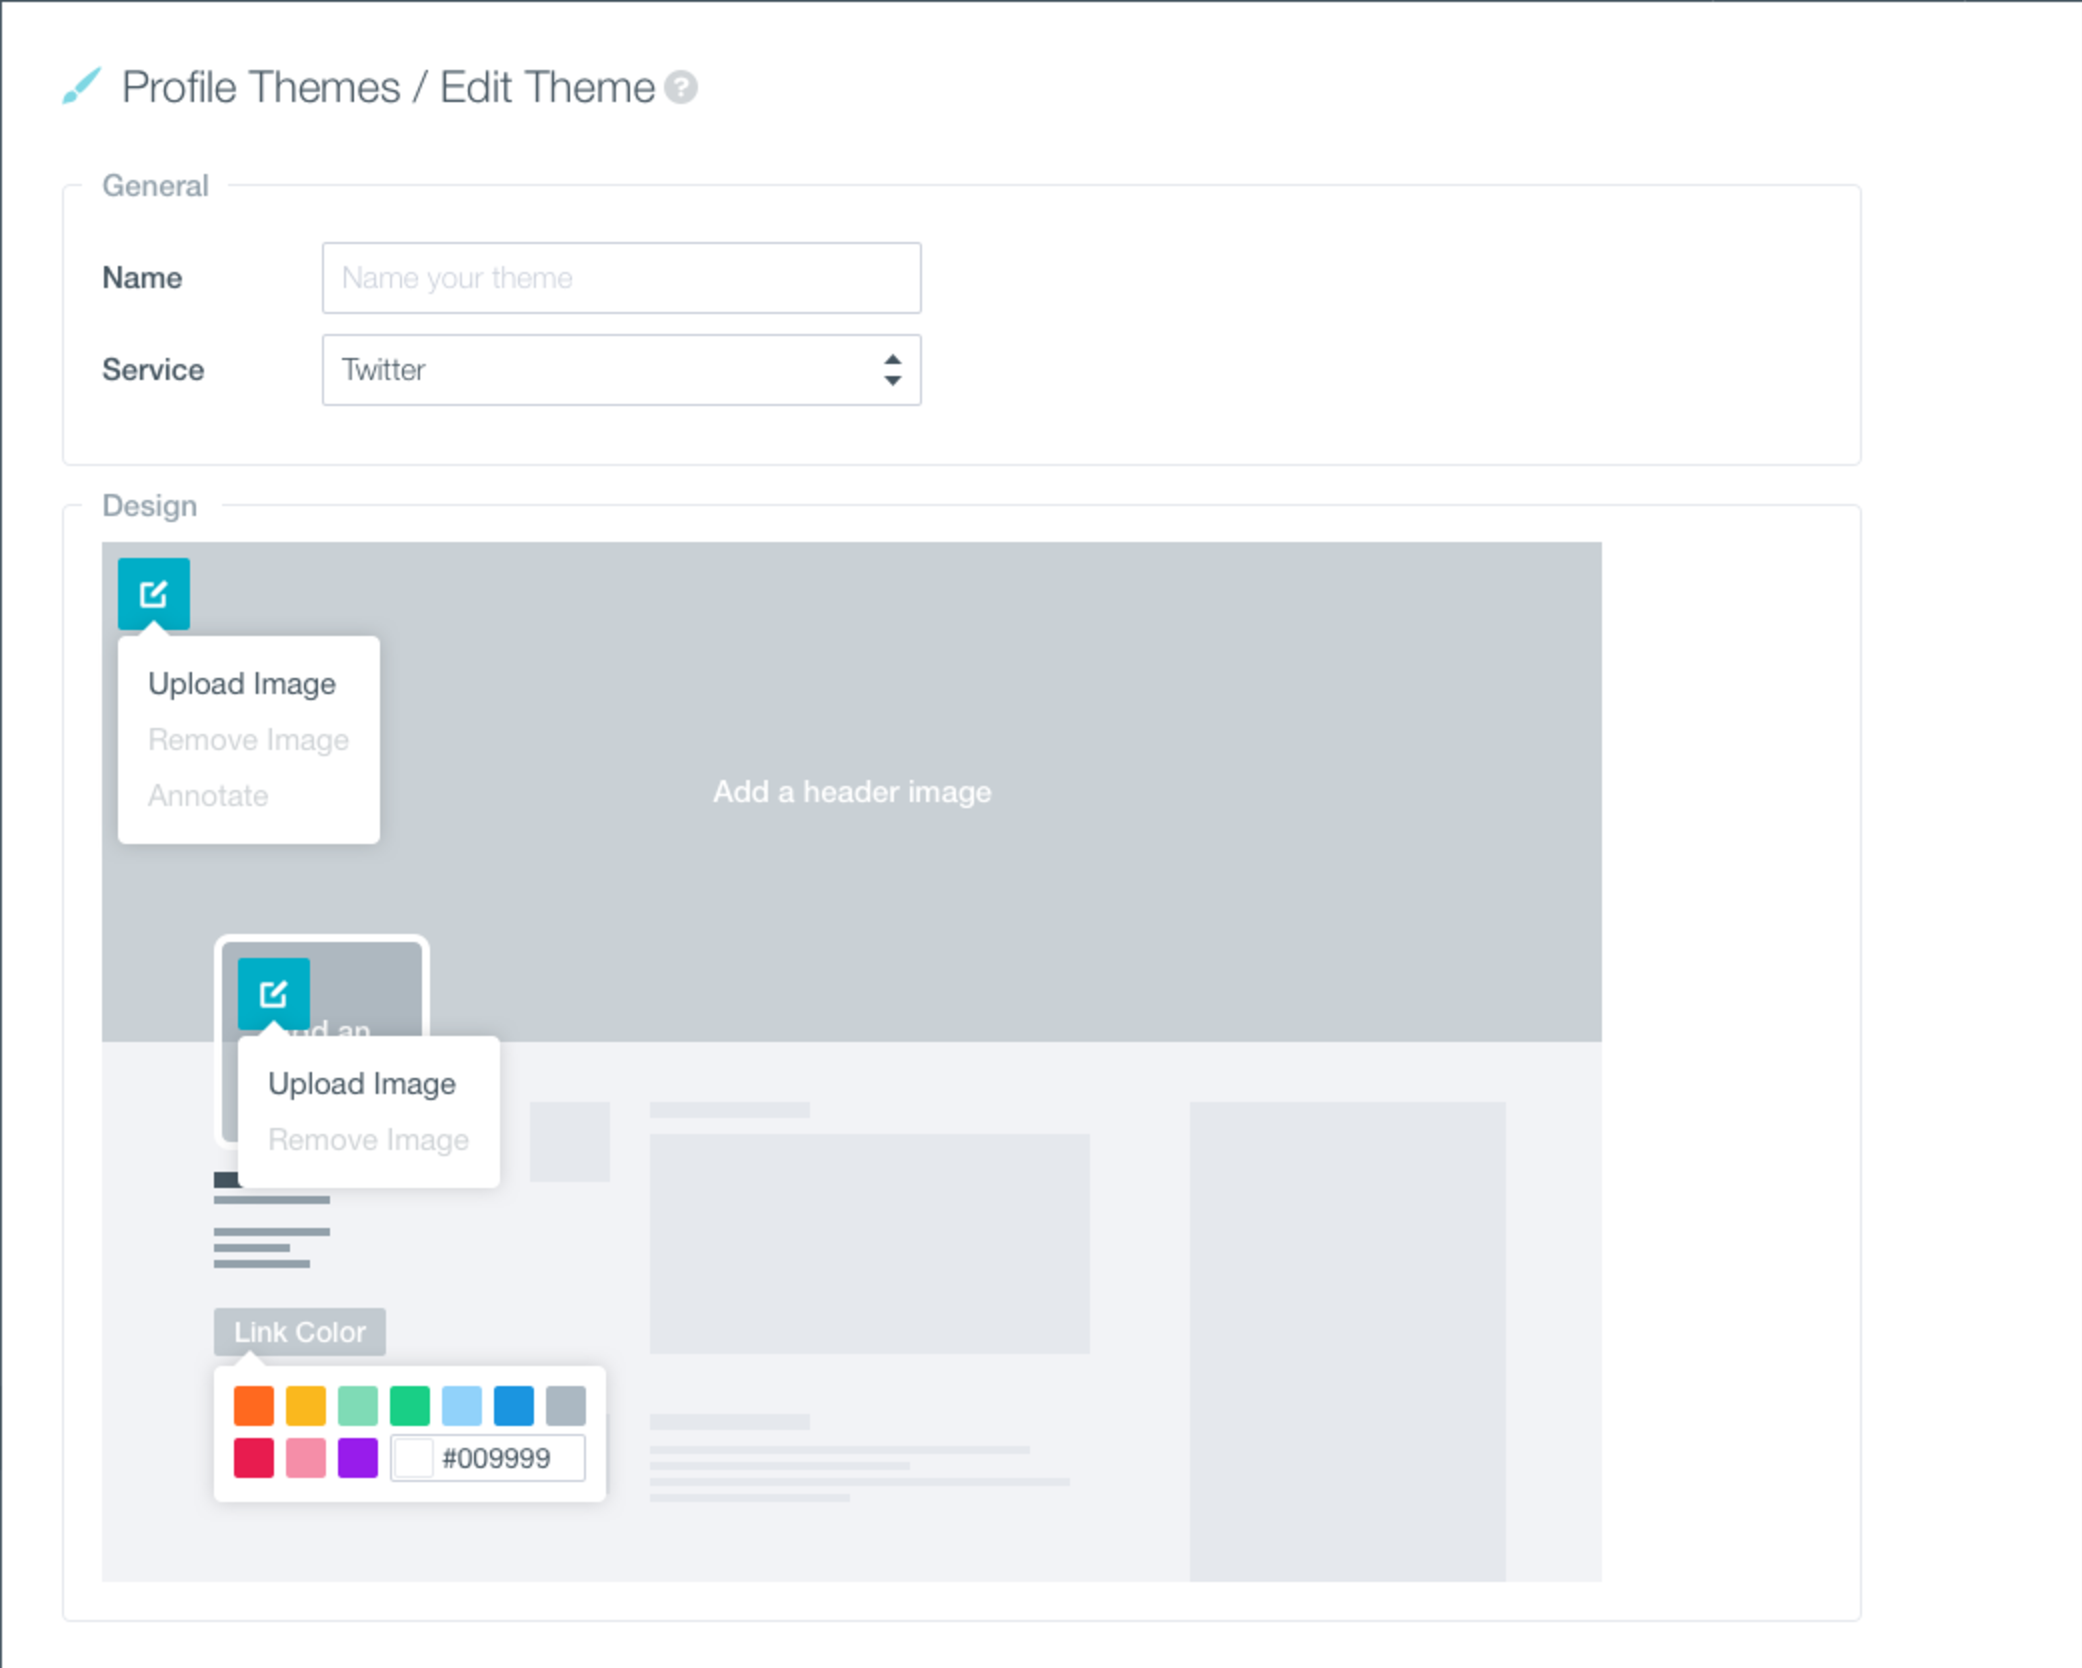
\includegraphics[width=0.6\textwidth]{Figuren/EditThemeMockup.png}
	\caption{Mockup van de editeerpagina \cite{EditThemeMockup}} %\cite{Pouladzadeh}
	\label{fig:EditTheme}
\end{figure} 

\chapter{Omschrijving bachelorproef}
\vspace{-3cm}
Deel van de stageopdracht is het verwerken van afbeeldingen om als omslagfoto of avatar te gebruiken. Hierbij is het de bedoeling dat klanten afbeeldingen kunnen uploaden die dan als omslagfoto en/of avatar zullen dienen.  Een thema, bestaande uit deze afbeeldingen en in sommige gevallen nog enkele andere variabelen zoals link kleur, info of naam van het profiel, kunnen ingesteld worden om op bepaalde tijdstippen actief te zijn. Klanten moeten in staat zijn tekst en KPI's op deze afbeeldingen te plaatsen vanuit de webapplicatie. De afbeeldingen moeten samengesteld kunnen worden door de gebruiker maar moeten nadien ook opnieuw gerenderd kunnen worden met aangepaste KPI's. Dit moet dus op de server gebeuren. 

Om afbeeldingen te annoteren is redelijk wat functionaliteit nodig. Ingegeven tekst moet eender waar op een afbeelding geplaatst kunnen worden maar moet ook gestyled kunnen worden. Gebruikers moeten alle basiseigenschappen van een stuk tekst kunnen aanpassen. Lettertype, kleur, lettergrootte, gewicht en uitlijning moeten allemaal ingesteld kunnen worden door gebruikers. Dit moet zowel clientside als serverside mogelijk zijn. Bibliotheken en technologie\"{e}n zullen onderzocht worden om dit te kunnen verwezenlijken.
\fi  

